%% TODO: insert high-level summary of this chapter

\section{Related Works}


  \subsection{Neural Approaches}

    \todo

    \subsubsection{Deep Object Pose Estimation}

      \todo
      \cite{DBLP:journals/corr/abs-1809-10790}

    \subsubsection{PoseCNN}

      \todo

  \subsection{Inverse Graphics}

    \todo[Picture, Analysis by Synthesis, Informed Sampler]


  \subsection{Bayesian Inference over Structured Scenes}

    Existing perspectives on Bayesian methods in vision systems operate under a
    fully-generative analysis-by-synthesis approach to modeling vision. This
    includes a full rendering pipeline and likelihood defined over 

    \subsubsection{Contact Graph Representation}

      \todo[FIG: Contact graph representation (maybe from Ben's poster?)]

    \subsubsection{Existential Doubt}

      \todo[FIG: NeurIPS figure]

    \subsubsection{LAFI}

      \todo[LAFI figure]
      \begin{figure}[t]
          \centering
          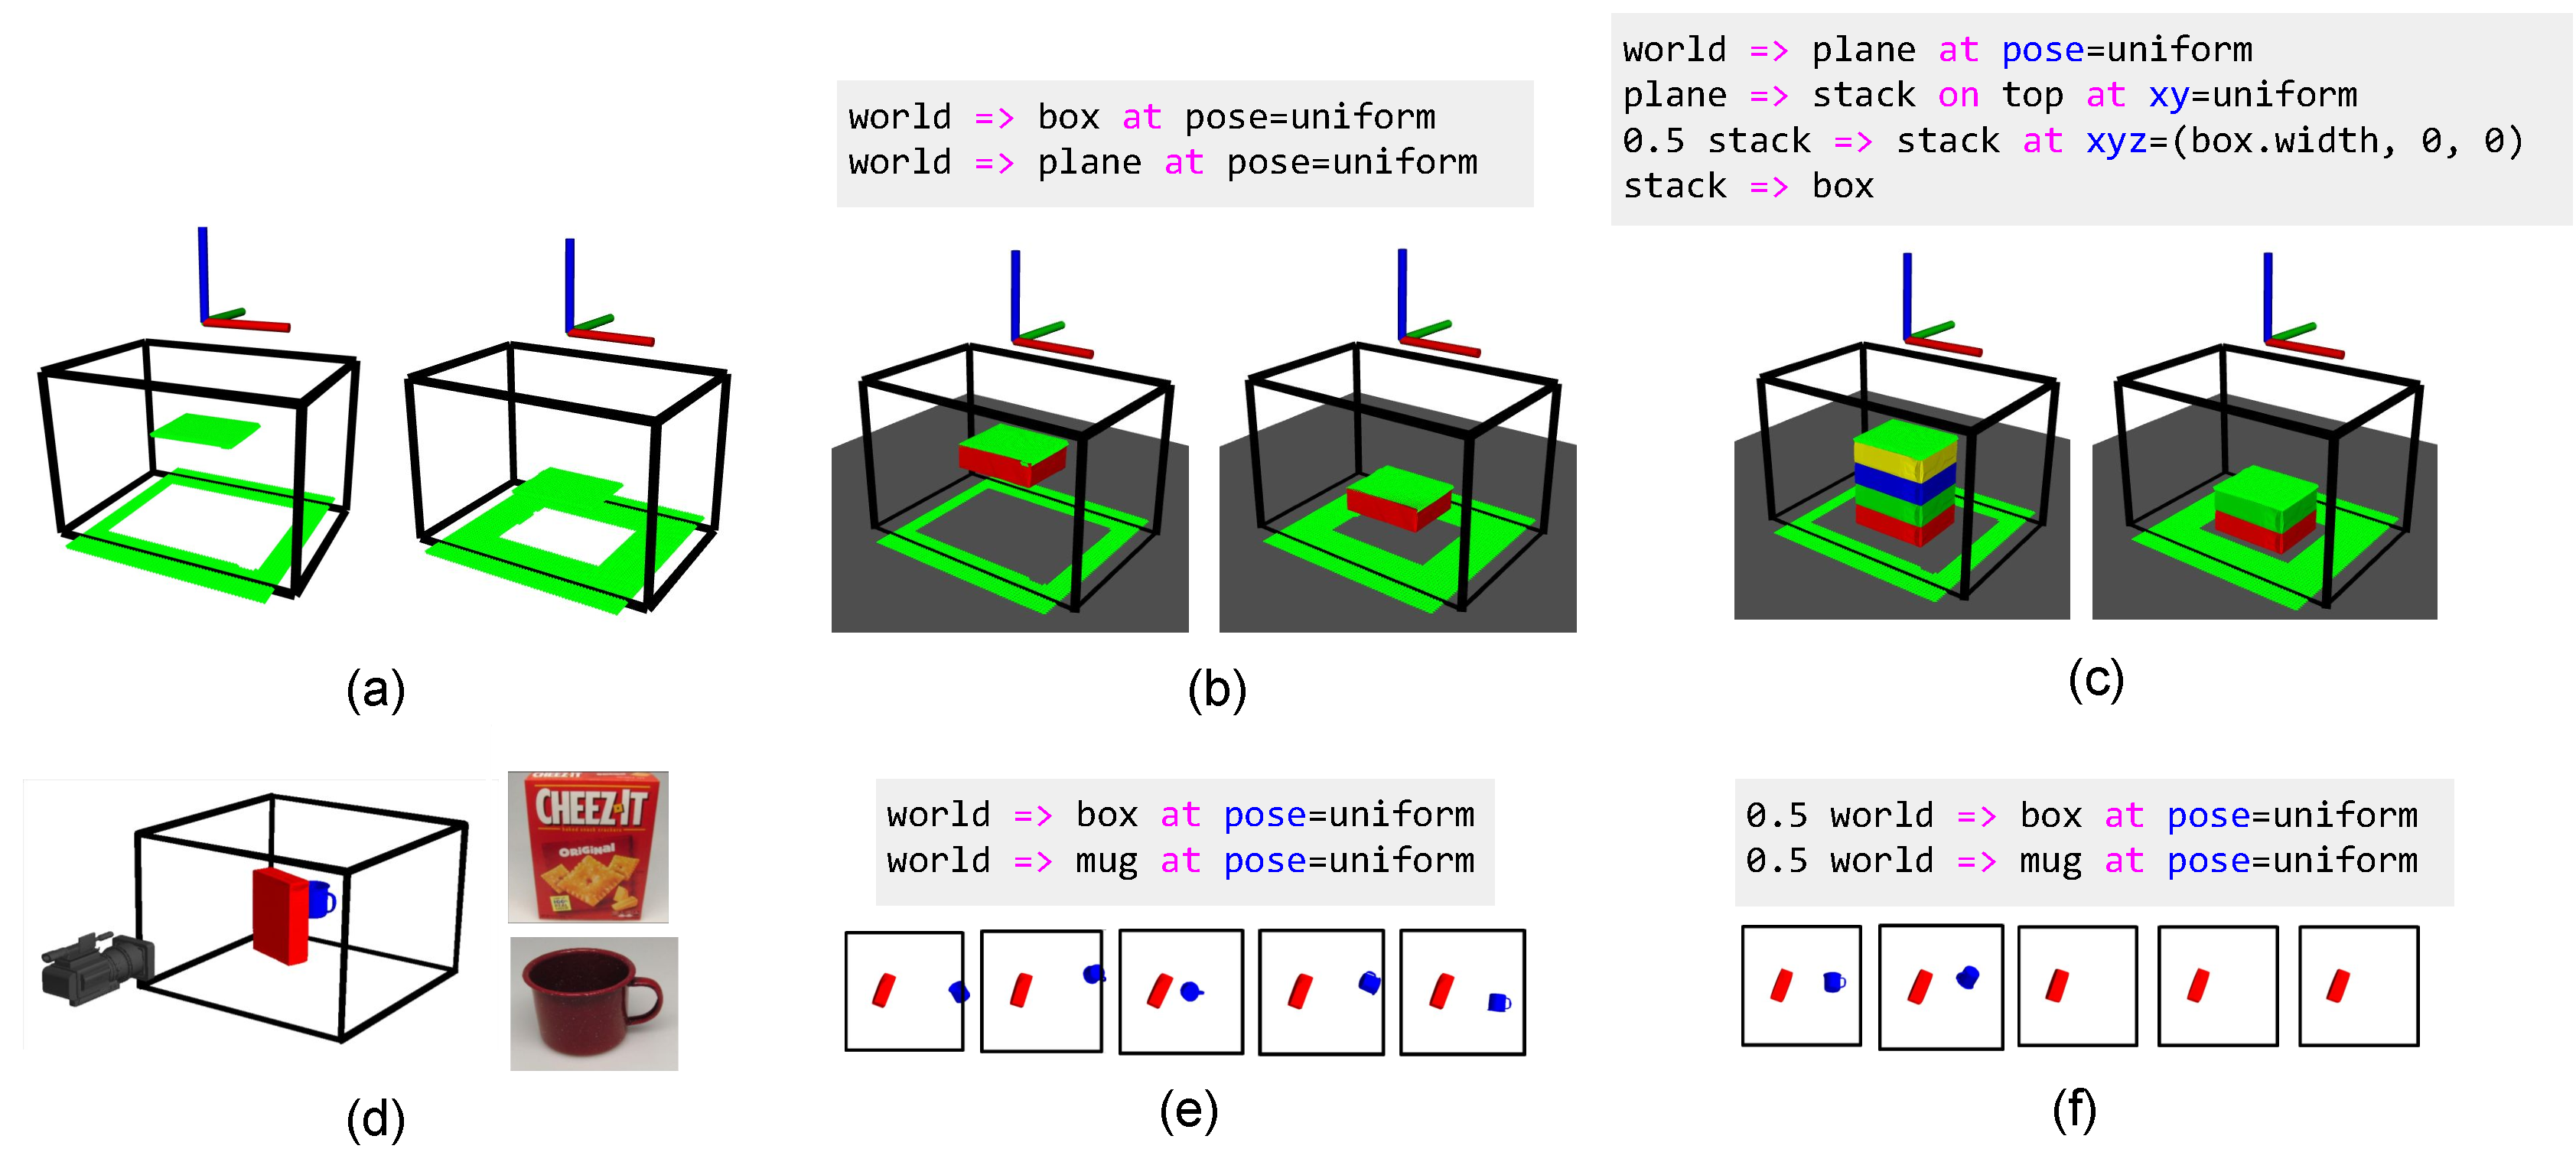
\includegraphics[width=\textwidth]{figures/lafi-fig.pdf}
          \caption{\small
            Two scenarios with prior knowledge specified as programs in our probabilistic scene description language.
            (a) shows two depth measurements made by a depth camera.
            (b) shows a program in which boxes have random poses in 3D space, and the resulting inferred pose of the box.
            (c) shows a program that assumes boxes are in stacks that rest on the floor, and the inferred number of boxes that explain the data for each observation.
            (d) shows another scenario, where a depth camera observes a box that is occluding a mug.
            (e) shows a program that asserts that both objects exist (but at unknown poses).
            The resulting inferences show the mug must exist somewhere behind the box to be consistent with this knowledge and the observation.
            (f) shows a program that allows for either object to not exist, and the resulting joint inferences about the mug's existence and pose.
            }
          \label{fig:results}
      \end{figure}
